\documentclass{beamer}

\usetheme{Berlin}

\usepackage{fontspec}
\usepackage{polyglossia}
\setmainlanguage{czech}

\usepackage{graphicx}
\usepackage{epstopdf}

\setlength{\unitlength}{0.5cm}

\title{Simulace SMP}
\author{Zdeněk Janeček \& Tomáš Cigler \& David Fiedler} 
\date{18.\,prosince 2015}

\begin{document}

\begin{frame} 
\titlepage
\end{frame}

\begin{frame} 
\frametitle{Zadání a úvod}
Vytvořte simulátor čtyřjádrového SMP a k němu:

\begin{itemize}
\item plánovač
\item synchronizaci procesů (semafory)
\item úlohu producent-konzument (poběží v osmi instancích)
\item rozhraní pro řízení procesoru a spuštěných úloh
\end{itemize}

\end{frame}


\begin{frame} 
\frametitle{Návrh implementace}

\begin{itemize}
\item start podobný jako start systému
\item inicializace systému obsluh přerušení
\item běh procesoru - jedna INIT úloha
\item inicializace úloh producent-konzument do plánovače
\item plánování na základě přerušení a časového kvanta (Round Robin)
\end{itemize}

\end{frame}

\begin{frame} 
\frametitle{Rozhraní}

Konzole jako ovládací a monitorovací rozhraní:

\begin{itemize}
\item exit: vypne program
\item start: spustí úlohu
\item help: ukáže nápovědu
\item show: ukáže informace o~běžících procesech,čekajících procesech a obsazenosti CPU
\item state: zobrazí aktuální chybu výpočtu v~úlohách. Tato funkce je volána pravidelně.
\item pause-core: pozastaví jádro procesoru
\item resume-core: znovu spustí jádro procesoru
\end{itemize}

\end{frame}

\begin{frame} 
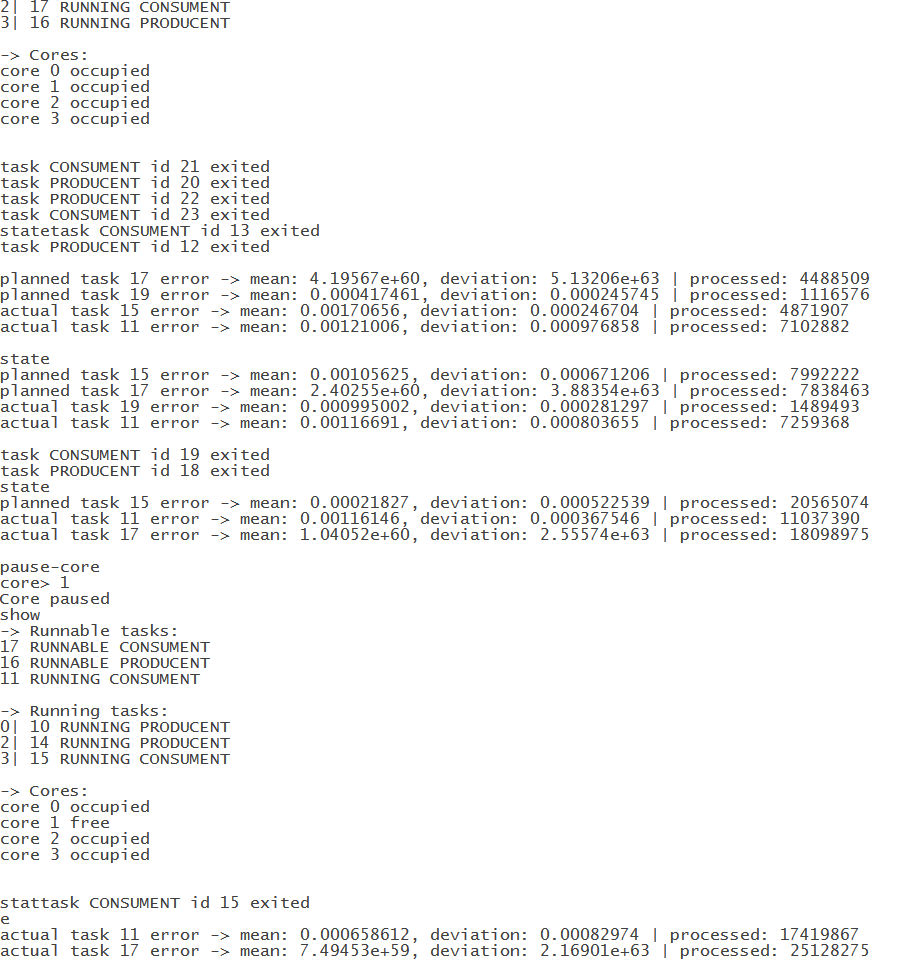
\includegraphics[height=\textheight]{obrazky/screen.png}

\end{frame}

\begin{frame} %[fragile]
\frametitle{Procesor - přerušení}

\end{frame}

\begin{frame} %[fragile]
\frametitle{Plánovač}

\end{frame}

\begin{frame} %[fragile]
\frametitle{Úlohy}
\begin{itemize}
\item Dodělám zítra ráno
\end{itemize}
\end{frame}

\begin{frame} 
\frametitle{Výsledky a závěr}

\end{frame}

\end{document}
